\documentclass[11pt,letterpaper]{article}
\usepackage[utf8]{inputenc}

%----- Configuración del estilo del documento------%
\usepackage{epsfig,graphicx}
\usepackage[left=2cm,right=2cm,top=1.8cm,bottom=2.3cm]{geometry}
\usepackage{fancyhdr}
\usepackage{lastpage}
\usepackage{url}
\pagestyle{fancy}
\fancyhf{}
\rfoot{\textit{Página \thepage \hspace{1pt} de \pageref{LastPage}}}


%------ Paquetes matemáticos básicos --------%
\usepackage{amsmath}
\usepackage{amssymb}
\usepackage{amsthm}

\usepackage[spanish]{babel}
\usepackage{graphicx}
\usepackage{hyperref}

\usepackage{tabularx}
\usepackage{xcolor}
\usepackage[table]{xcolor}
\usepackage{colortbl}
\usepackage{array, multirow, multicol, tabularx}
\usepackage{tcolorbox}
\newtheorem{theorem}{Theorem}[section]
\newtheorem{corollary}{Corollary}[theorem]
\newtheorem{lemma}[theorem]{Lemma}

%------si-------%
\definecolor{B}{HTML}{FFFFFF}
\definecolor{G}{HTML}{5e5e5e}
\definecolor{R2}{HTML}{d53d40}
\definecolor{A2}{HTML}{034190}
\definecolor{V2}{HTML}{7faa50}
\newcommand{\R}{\mathbb{R}}
\newcommand{\C}{\mathcal{C}}
\newcommand{\N}{\mathbb{N}}
\newcommand{\Z}{\mathbb{Z}}
\newcommand{\Q}{\mathbb{Q}}
\renewcommand{\theenumi}{\Roman{enumi}}
\renewcommand{\labelenumi}{{\theenumi}.}

\begin{document}

%------ Encabezado -------- %

\begin{center}
    \begin{minipage}{3cm}
    	\begin{center}
    		\includegraphics[height=3.4cm]{logo_unam.png}
    	\end{center}
    \end{minipage}\hfill
    \begin{minipage}{10cm}
    	\begin{center}
    	\textbf{\large Universidad Nacional Autónoma de México}\\[0.1cm]
        \textbf{Facultad de Ciencias}\\[0.1cm]
        \textbf{C\'alculo II}\\[0.1cm]
        Resumen del Curso\\[0.1cm]
         El\'ias L\'opez Rivera\\[0.1cm]
        \texttt{ elias.lopezr\,@ciencias.unam.mx }\\[0.1cm]
        Fecha:\,\,06/07/2025
    	\end{center}
    \end{minipage}\hfill
    \begin{minipage}{3cm}
    	\begin{center}
    		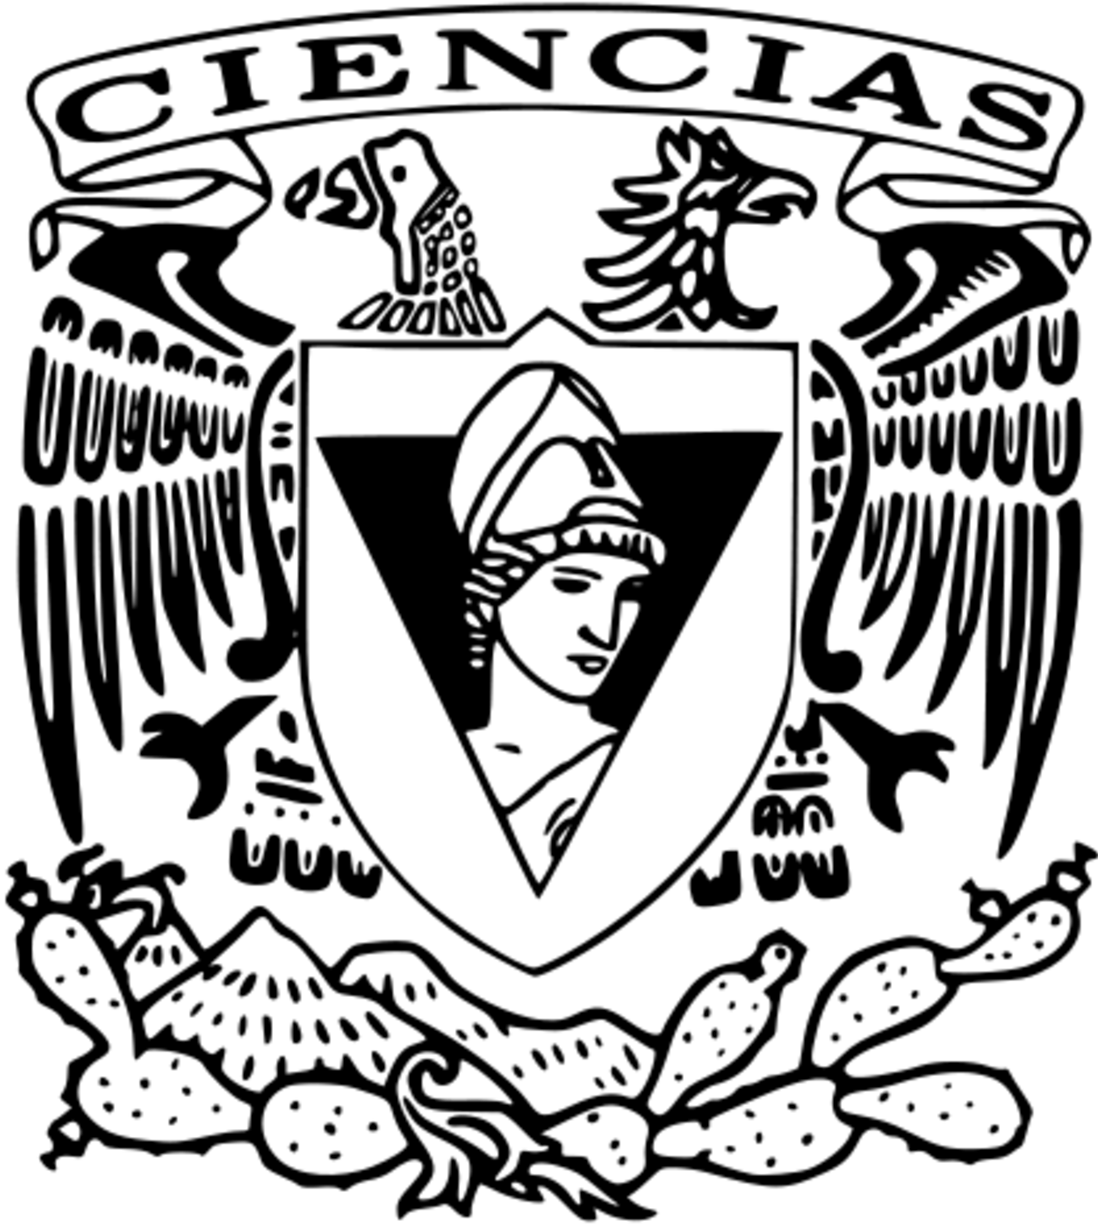
\includegraphics[height=3.4cm]{Logo_FC.png}
    	\end{center}
    \end{minipage}
\end{center}

\rule{17cm}{0.1mm}

%------ Fin de encabezado -------- %
\,\\
\begin{tcolorbox}[
	title = \textcolor{black}{\textcolor{white}{C\'alculo 2}},]
\textit{El siguiente documento es una recopilaci\'on de los teoremas,problemas de examenes,ejemplos y solcuiones m\'as 
importantes expuestos durante el curso de C\'alculo II, del profesor Javier Páez Cardeas, de la facultad de ciencias de la unam }
\end{tcolorbox}
\section*{Teorema de integrabilidad de Lebesgue}
Antes de poder demostrar este teorema necesitamos introducir 3 conceptos importantes que se usaran durante la prueba.
\subsection*{Conjuntos Nulos}
\begin{tcolorbox}[
	title = \textcolor{black}{\textcolor{white}{Definici\'on 1}},]
\textit{Decimos que un conjunto $A\subset \R$ es nulo si dado $\epsilon>0$, existe una coleccio\'n contable $\{(a_k,b_k)\}_{k=1}^{\infty}$, de intervalos abiertos tales que:\,\\
\,\\
\begin{equation*}
    Z\subseteq\,\bigcup_{k=1}^{\infty}\,(a_k,b_k)\,\,\,\,y\,\,\,\,\sum_{k=1}^{\infty}\,(b_k-a_k)\leq \epsilon
\end{equation*}}
\end{tcolorbox}\,\\
Partiendo de lo anterior es fácil demostrar los siguientes hechos:
\begin{tcolorbox}[
	title = \textcolor{black}{\textcolor{white}{Teorema 1}},]
\textit{\textbf{Union de conjuntos nulos}
\begin{enumerate}
    \item Si $Z_1$, $Z_2$ son conjuntos nulos entonces $Z_1\cup Z_2$ es un  conjunto nulo
\item Si $Z_n$ es un conjunto nulo para toda $n\in \N$, demostrar que $\bigcup_{n=1}^{\infty}\,Z_n$, es un conjunto nulo
\end{enumerate} }
\end{tcolorbox}
\begin{proof}\,\\
    \,\\
    \textbf{1}\,\,Tenemos que como $Z_1$ y $Z_2$ son nulos, entonces para $\frac{\epsilon}{2}>0$, existen $\{J^{1}_{k}|\,k\in \N\}$ y $\{J^{2}_{k}|\,k\in \N\}$, tales que
    $\sum_{k\in \N}\,|J^1_{k}|<\frac{\epsilon}{2}$ y $\sum_{k\in \N}\,|J^2_{k}|<\frac{\epsilon}{2}$, tenemos que $\{J^{1,2}_{k}|k\in \N\}:=\{J^1_{k}|k\in \N\}\cup\{J^2_{k}|k\in \N\}$, es un conjunto contable
    de intevalos, luego tenemos que $Z_1\cup Z_2\subset \bigcup\,_{k\in \N}\,J^{1,2}_{k}$, ademas que \\$\sum_{k\in \N}\,|J_k^{1,2}|\leq\sum_{k\in \N}\,|J^1_{k}|+\sum_{k\in \N}\,|J^2_{k}|
    \leq \frac{\epsilon}{2}+\frac{\epsilon}{2}=\epsilon$
    \newpage
    \,\\
    \textbf{2}\,\,Dada $\epsilon>0$ y $n\in \N$ existe $\{J^n_{k}|\,k\in \N\}$ tal que $Z_n\subset\bigcup_{k\in \N}\,\,J^{n}_{k}$ y $\sum_{k\in \N}\,|J^n_{k}|<\frac{\epsilon}{2^n}$, definimos\\
    $\{J^{n}_{k}|n,k\in \N\}=\bigcup_{n\in \N}\,\{J^n_{k}|k\in \N\}$, es claro que $\{J^{n}_{k}|n,k\in \N\}$ es un conjunto contable de intervalos abiertos, ademas tenemos que
    $\bigcup_{n=1}^{\infty}\,Z_n\subset\,\bigcup_{k,n\in \N}\,J^{n}_{k}$, luego finalmente tenemos que:\,\\
    $\sum_{k,n\in \N}\,|J^n_{k}|\leq \sum_{k\in \N}\,\frac{\epsilon}{2^n}=\epsilon$
\end{proof}\,\\
\begin{tcolorbox}[
	title = \textcolor{black}{\textcolor{white}{Teorema 2}},]
\textit{\textbf{Ejemplos de subconjuntos nulos}
\begin{enumerate}
    \item Si $Z\subset \R$ es finito, entonces $Z$ es nulo
\item $\Q\subset \R$ es nulo
\item $\emptyset$ es nulo
\end{enumerate} }
\end{tcolorbox}
\begin{proof}\,\\
    \,\\
    \textbf{1}\,Se sigue del hecho de que $Z$ no tiene puntos de acumulaci\'on ,por tanto para todo $z\in \Z$ existe una vecindad $V_{x}(\epsilon)$ tal que $V_{x}(\epsilon)\cap Z-\{x\}=\emptyset$, tome estas vecindades como intervalos y rellene su coleccion contable con $\emptyset$, se dejan los detalles
    de la demostraci\'on al lector\,\\
    \,\\
    \textbf{2}\,La demostraci\'on puede encontrarse en el Bartle (p\'agina 267).\,\\
    \,\\
    \textbf{3}\,Se sigue directamente por vacuidad
\end{proof}
\subsection*{Oscilaciones de una funci\'on}
\begin{tcolorbox}[
	title = \textcolor{black}{\textcolor{white}{Definici\'on 2}},]
\textit{Sea $f:A\rightarrow \R$ una funcion acotada. si $S\subset A\subset \R$, definimos la Oscilaci\'on de 
$f$ en $S$ como:\,\\
\,\\
\begin{equation*}
        W(f,S):=sup\{|f(x)-f(y)|:x,y\in S\}
\end{equation*}\,\\
Si $c\in A$, la oscilaci\'on de $f$ en $c$, se define como:\,\\
\,\\
\begin{equation*}
    w(f,c):=inf\{W(f;V_r(c)):r>0\}=\lim_{r\rightarrow 0+}\,W(f;V_r(c))
\end{equation*}}
\end{tcolorbox}
\newpage
\,\\
De la definici\'on podemos deducir el siguiente teorema:
\begin{tcolorbox}[
	title = \textcolor{black}{\textcolor{white}{Teorema 3}},]
\textit{Si $f:A\rightarrow\R$ esta acotada y $x_0\in A$, entonces $f$ es continua en $x_0$ si y s\'olo si $w(f;x_0)=0$}
\end{tcolorbox}
\begin{proof}\,\\
    \,\\
   Primero demostremos que:\\
\begin{equation*}
    w(f,x_0)= inf \{ sup \{ |\,\textit{f}\,(x)- \textit{f}\,(y)| :x,y \in V_\delta (x_0)\cap A, \delta>0\}\}
\end{equation*}\\
Sea $\delta>0$, definimos:\\
\begin{equation*}
    g(\delta):=sup \{ |\,\textit{f}\,(x)- \textit{f}\,(y)\,| :x,y \in V_\delta (x_0)\cap A \}
 \end{equation*}\\
Como $0<g(\delta)$ $\forall\, \delta>0$, sabemos que existe $inf\{g[I]\}$, con $I:=(0,\infty)$.\\
\,\\
Sea $\epsilon>0$ $\exists\,t>0$ tal que:\\
\begin{equation*}
    g(t)<inf\{g[I]\}+\epsilon
\end{equation*}\\
finalmente sea x$\in (0,t)$, como $x<t$, se tiene que  $g(x)<g(t)$
concluimos que:\\
\begin{equation*}
    inf\{g[I]\}-\epsilon<g(x)<inf\{g[I]\}+\epsilon
\end{equation*}\\
Es decir $\forall\,\epsilon>0$ $\exists\,t>0$ tal que:\\
\,\\
Si $x\in(0,t)$, entonces: $g(x)\in V_\epsilon(inf\{g[I]\})$
por tanto: \\
\begin{equation*}
    w(f,x_0)= inf \{ sup \{ |\,\textit{f}\,(x)- \textit{f}\,(y)\,| :x,y \in V_\delta (x_0)\cap A, \delta>0\}\}
\end{equation*}\\
$\Longrightarrow$) Tomando en cuenta que \textit{f} es continua en $x_0$, la condici\'on continua de Cauchy nos asegura la existencia de $\delta_1 > 0$ tal que, si $x,y\in V_{\delta_1} (x_0)\cap A$ se cumple que $|\,\textit{f}\,(x) - \textit{f\,}(y)\,|<\epsilon$, para alg\'un $\epsilon >0$\\ 
Luego tenemos, por la condici\'on de supremo:\\
\begin{equation*}
 sup \{ |\,\textit{f}\,(x)- \textit{f}\,(y)\,| :x,y \in V_{\delta_1} (x_0)\cap A\}< \epsilon 
\end{equation*}\\
Finalmente, aplicamos la condici\'on de \'infimo a lo anterior:\\
\begin{equation*}
    w(f,x_0)<\epsilon
\end{equation*}\\
Debido a que 0 es cota inferior del conjunto $g[I]$:\\
\begin{equation*}
    0\leq w(f,x_0)<\epsilon
\end{equation*}\\
como $\epsilon$ es arbitrario, conlcuimos que:\\
\begin{equation*}
    w(f,x_0)=0
\end{equation*}\\
$\Longleftarrow$) Ahora, suponiendo que $w(f,x_0)=0$, sabemos , por la condici\'on de \'infimo que:\\
\,\\
Sea $\epsilon>0$, existe $\delta_1>0$ tal que:\\
\begin{equation*}
    sup \{ |\textit{f}\,(x)- \textit{f}\,(y)| :x,y \in V_{\delta_1} (x_0)\cap A\}<w(f,x_0) + \epsilon= \epsilon
\end{equation*}\\
Luego aplicando la condicion de supremo, fijamos x=$x_0$, tomamos y $\in V_{\delta_1}(x_0)\cap A$ tal que:\\
\begin{equation*}
    |\,\textit{f}\,(x_0)-\textit{f}\,(y)\,|<\epsilon
\end{equation*}\\
Como \'epsilon es arbitrario, se cumple la condici\'on de continuidad, por tanto \textit{f} es continua en $x_0$.
\end{proof}\,\\
\begin{tcolorbox}[
	title = \textcolor{black}{\textcolor{white}{Teorema 4}},]
\textit{Si $f:[a,b]\rightarrow\R$ esta acotada, entonces $D:=\{c\in [a,b]:w(f,c)>0\}=\bigcup_{k\in \N}\,H_k$, donde 
$H_k=\{c\in [a,b]:w(f,c)>\frac{1}{2^k}\}$}
\end{tcolorbox}
\begin{proof}\,\\
    \,\\
    Como $\displaystyle lim_{n\rightarrow \infty}\,\frac{1}{2^n}=0$, si tomamos $c\in D$, entonces $w(f,c)=\epsilon>0$, por tanto existe
    $k\in \N$ tal que si $n\geq k$ entonces $\frac{1}{2^n}<\epsilon=w(c,f)$, por tanto $c\in H_n$ para alg\'un $n\in \N$, se concluye que $c\in\bigcup_{k\in \N}\,H_k$, por tanto $D\subseteq \bigcup_{k\in \N}\,H_k$, la otra contecni\'on es trivial, debido
    al teorema $3$ tenemos que $\bigcup_{k\in \N}\,H_k$ es el conjunto de discontinuidades de $f$ en $[a,b]$
\end{proof}
\subsection*{Medidas $\delta$ y particiones fina-$\delta$}
\begin{tcolorbox}[
	title = \textcolor{black}{\textcolor{white}{Definici\'on 3}},]
\textit{Sea $A\subset \R$ una medida $\delta$ en $A$ es una funci\'on estrictamente positiva en $A$, sea $P:=\{(I_k,t_k)\}_{k\in \N_n}$, esta se directamente
fina-$\delta$ si cumple que:\,\\
\begin{equation*}
    t_i\in I_i\subseteq [t_i-\delta(i),t_i+\delta(i)]\,\,\,\,\forall i\in \N_n
\end{equation*}}
\end{tcolorbox}\,\\
De la definici\'on se desprende el siguiente teorema el cual no demostraremos ya que escapa del proposito del texto:
\begin{tcolorbox}[
	title = \textcolor{black}{\textcolor{white}{Teorema 5}},]
\textit{Si $\delta$ e suna medida definida en $[a,b]\subset \R$, entonces existe
una partici\'on fina-$\delta$ de $[a,b]$}
\end{tcolorbox}
\newpage
\,\\
\subsection*{Enunciado y demostraci\'on}
\begin{tcolorbox}[
	title = \textcolor{black}{\textcolor{white}{Teorema de integrabilidad de Lebesgue }},]
\textit{Sea $f:[a,b]\rightarrow \R$ una funci\'on acotada, esta es Riemann integrable si y solo si su conjunto de discontinuidades es nulo}
\end{tcolorbox}
\begin{proof}\,\\
    \,\\
    $\Rightarrow)$\,Si $f$ es continua en $[a,b]$, entonces $f$ es continua y por tanto su conjunto de discontinuidades es nulo pues $\emptyset$ es nulo por el teorema 2, por
    tanto sea $D$ definido en el teorema 4, el conjunto de discontinuidades de $f$ en $[a,c]$, supongamos que este es no vacio,como estamos considerando que $D=\bigcup_{l\in \N}\,H_l\neq \emptyset$  por tanto existe $K\in \N$ tal que $H_k\neq \emptyset$, tomemos $\frac{\epsilon}{2^k}>0$, por el criterio de Riemann, existe una partici\'on $P_k:=\{[x^k_{i-1},x^k_{i}]\}_{i=0}^{n(k)}$, tal que:\,\\
    \begin{equation*}
        \sum_{i=1}^{n(k)}\,(M^k_i-m^k_i)\,(x^k_{i}-x^k_{i-1})<\frac{\epsilon}{2^k}
    \end{equation*}\,\\
    Donde $M^k_i$ y $m^k_i$ son el respectivo infimo y supremo de la partici\'on, ,, como $H_k\subset P$ para toda $l\in \N$, existe $(x^k_{i-1},x^k_{i})$ tal que $(x^k_{i-1},x^k_{i})\cap H_k\neq \emptyset$, sea
    $x\in (x^k_{i-1},x^k_{i})\cap H_k$, entonces existe $r>0$ tal que $V_r(x)\subseteq (x^k_{i-1},x^k_{i})$, se sigue que:\,\\
    \begin{equation*}
        \frac{1}{2^k}\leq w(f,x) \leq W(f,V_r(x))\leq M^k_i-m^k_i
    \end{equation*}\,\\
    Si hacemos $\sum^{'}$ la sumatoria sobre todos los $i$ tal que $H_k\cap (x^k_{i-1},x^k_{i})\neq \emptyset$, tenemos que:\,\\
    \begin{equation*}
        \frac{1}{2^k}\,\sum^{'}\,(x^k_{i}-x^k_{i-1})\leq \sum_{i=1}^{n(k)}\,(M^k_i-m^k_i)\,(x^k_{i}-x^k_{i-1})<\frac{\epsilon}{2^k}\implies \sum^{'}\,(x^k_{i}-x^k_{i-1})\leq \epsilon
    \end{equation*}\,\\
    Tenemos que $H_K\neq \emptyset$ esta totalmente contenido en una subpartici\'on $P'$ fininita tal que la longitud de sus intervalos es menor a $\epsilon$, por el teorema 2 $H_k$ es un conjunto nulo, por tanto $D=\bigcup_{l\in \N}\,H_l$
    es un subconjunto nulo por el teorema 1\,\\
    \,\\
    $\Leftarrow$)\,Sea $|f(x)|\leq M$ para $x\in [a,b]$ y supongamos que $D$ es un conjunto nulo, entonces dado $\epsilon>0$, existe un conjunto contable $\{J_k\}_{k\in \N}$ de intervalos abiertos con $D\subseteq\,\bigcup_{k\in \N}\,J_k$ y $\sum_{k\in \N}\,|J_k|\leq \frac{\epsilon}{4M}$, definimos $\delta$ una medida sobre $[a,b]$ de la siguiente manera:\,\\
    \begin{enumerate}
        \item \textbf{i)}\,\,Si $t \notin D$, entonces $f$ es continua en $t$ y existe $\delta(t)>0$ tal que si $x\in V_{\delta(t)}(t)$, entonces $|f(x)-f(t)|<\frac{\epsilon}{4(b-a)}$,de donde:\,\\
        \begin{equation*}
            0\leq M_i-m_i\leq \frac{\epsilon}{2(b-a)}
        \end{equation*}
        \item \textbf{ii)}\,\,Si $t\in D$, se elige $\delta(t)>0$ tal que $V_{\delta(t)}(t)\subseteq J_k$ para alguna $k\in \N$, para estos valores se cumple que $0\leq M_t-m_t\leq 2M$
    \end{enumerate}\,\\
    Por tanto por el teorema 5 existe $P:=\{([x_{i-1},x_i],t_i)\}_{i=1}^{n}$ partici\'on fina-$\delta$, separamos los indices $i$ en los siguientes dos conjuntos disjuntos:\,\\
    \begin{equation*}
        S_c:=\{i:t\notin D\}\,\,\,\,S_d:=\{i:t_i\in D\}
    \end{equation*}\,\\
    Como $P$ es fina-$\delta$ se tiene que $[x_{i-1},x_i]\subseteq V_{\delta(t_i)}(t_i)$, luego tenemos que $M_i-m_i\leq M_{t_i}-m_{t_i}$, por tanto si $i\in S_c$ entonces $M_i-m_i\leq \epsilon$, en tanto que si $i\in S_d$, se tiene que $M_i-m_i\leq 2M$, luego
    tenemos que la collecci\'on de intervalos $[x_{i-1},x_i]$ con $i\in S_d$ esta contenida en la union arbitraria de $\{J_k\}_{k\in \N}$ cuya longitud es menor a $\frac{\epsilon}{4M}$, finalmente se sigue que:\,\\
    \begin{align*}
        \sum_{i=1}^n\,(M_i-m_i)(x_i-x_{i-1})=\sum_{i\in S_c}\,(M_i-m_i)\,(x_i-x_{i-1})+\sum_{i\in S_d}\,(M_i-m_i)\,(x_i-x_{i-1})\,\\
        \,\\
        \leq \sum_{i\in S_c}\,\frac{\epsilon}{2(b-a)}\,(x_i-x_{i-1})+\sum_{i\in S_d}\,2M\,(x_i-x_{i-1})\leq \frac{\epsilon\,(b-a)}{2(b-a)}+\frac{2M\epsilon}{4M}=\frac{\epsilon}{2}+\frac{\epsilon}{2}=\epsilon
    \end{align*}\,\\
    Como $\epsilon>0$ fue arbitrario se concluye que $f\in R[a,b]$
\end{proof}
\end{document}